\documentclass[11pt]{article}
% Shared packages, colours, TikZ styles and macros for the OrbiBot V1 report.

\usepackage[T1]{fontenc}
\usepackage{amsmath}
\usepackage{graphicx}
\usepackage{booktabs}
\usepackage{array}
\usepackage{xcolor}
\usepackage{url}
\usepackage{cite}
\usepackage{tikz}
\usepackage{pgfplots}
\usepackage[hidelinks]{hyperref}

\pgfplotsset{compat=1.18}
\usetikzlibrary{arrows.meta, positioning, fit, calc, shapes.geometric, backgrounds,
  decorations.pathreplacing}

\graphicspath{{../media/}}

% One palette for every figure: a layer has one colour everywhere.
\definecolor{mcu}{HTML}{E8F1FB}       % STM32 and firmware
\definecolor{mcuedge}{HTML}{2F6DB5}
\definecolor{host}{HTML}{EAF6EC}      % Raspberry Pi and ROS 2
\definecolor{hostedge}{HTML}{2E7D32}
\definecolor{ui}{HTML}{FFF4E0}        % dashboard and agent
\definecolor{uiedge}{HTML}{C77700}
\definecolor{hw}{HTML}{F1F1F1}        % hardware
\definecolor{hwedge}{HTML}{555555}
\definecolor{warn}{HTML}{FDECEC}
\definecolor{warnedge}{HTML}{B3261E}

\tikzset{
  >={Stealth[length=2mm]},
  box/.style={draw, rounded corners=2pt, align=center, font=\footnotesize,
              minimum height=7mm, inner sep=3pt},
  mcubox/.style={box, fill=mcu, draw=mcuedge},
  hostbox/.style={box, fill=host, draw=hostedge},
  uibox/.style={box, fill=ui, draw=uiedge},
  hwbox/.style={box, fill=hw, draw=hwedge},
  warnbox/.style={box, fill=warn, draw=warnedge},
  group/.style={draw, dashed, rounded corners=3pt, inner sep=6pt},
  grouplabel/.style={font=\scriptsize\itshape, anchor=north west},
  flow/.style={->, thick},
  dataflow/.style={->, thick, densely dashed},
  lbl/.style={font=\scriptsize, midway, fill=white, inner sep=1pt},
}

% A ROS 2 topic, frame or code name, typeset as written (underscores included).
\newcommand{\topic}[1]{\texttt{\detokenize{#1}}}


\begin{document}

% ---------------------------------------------------------------------------
% Title block
\thispagestyle{empty}
\begin{tcolorbox}[colback=accent, colframe=accent, arc=3pt, left=14pt, right=14pt, top=14pt, bottom=12pt]
  \color{white}\sffamily\raggedright
  {\small Technical report \quad$\cdot$\quad Version 1.0 \quad$\cdot$\quad October 2026}\par\vspace{8pt}
  {\LARGE\bfseries OrbiBot V1: A Mecanum Mobile Robot with Microcontroller-Level Real-Time Control, a ROS~2 Navigation Stack, and a Tool-Using LLM Agent}\par\vspace{6pt}
  {\large Design and Bench Evaluation}
\end{tcolorbox}

\vspace{4pt}
{\sffamily
\textbf{Jewel Nath}\quad{\color{muted}Independent researcher, Dhaka, Bangladesh}\\
{\small\color{muted}ORCID \href{https://orcid.org/0009-0002-6609-6378}{0009-0002-6609-6378}\quad$\cdot$\quad Code and data: \url{https://github.com/jewel-nath/orbibot-v1}}\par}

\vspace{6pt}
\begin{summarybox}{Abstract}
OrbiBot V1 is a four-wheel mecanum robot built by hand from a welded stainless-steel frame, a Raspberry Pi~5 running ROS~2 Jazzy, and an STM32F103 motor board running new open-source firmware. Its design rests on one split: every task with a deadline (a 100\,Hz PID loop per wheel, encoder counting, odometry, and a 2\,s command timeout) runs on the microcontroller under FreeRTOS, and everything that needs a map, a model or a network runs on the host.

On top of this base the robot maps with slam\_toolbox, fuses wheel odometry and a gyro in an extended Kalman filter, runs Nav2 with the MPPI controller in its omnidirectional mode, is driven from a browser dashboard, and exposes 58 robot tools to large language models through an HTTP interface, a terminal client and a Model Context Protocol server, with a safety layer on its direct motion tools.

The bench tests, made with the wheels off the ground, show chassis velocity within 1.3--9.3\,\% of the command, motors stopped between 1.82 and 2.12\,s after the last command against a 2\,s setting, a velocity clamp that held a 3\,m/s command to 1.02\,m/s, four motors within 0.1\,\% of each other at the speed limit, and a serial link that passed malformed-input tests after one critical fix. Mapping, navigation, the dashboard and the agent were run on the robot but not measured; the report states each such limit.

\smallskip
{\sffamily\small\textbf{Keywords:} mobile robots, mecanum wheels, ROS~2, embedded control, FreeRTOS, SLAM, Nav2, large language models, tool use, Model Context Protocol.}
\end{summarybox}

% ---------------------------------------------------------------------------
\section{Introduction}

Hobby-scale mobile robots can now run the same navigation software as research platforms. ROS~2~\cite{macenski2022ros2}, Nav2~\cite{macenski2020nav2} and slam\_toolbox~\cite{macenski2021slam} run on a single-board computer, and large language models (LLMs) can call software tools well enough to drive a robot through them~\cite{vemprala2024chatgpt}.

Putting these on one low-cost robot raises a practical problem. The host that runs mapping, planning, a web server and an LLM client is not real-time, yet the wheels need a steady control loop and a reliable way to stop. OrbiBot V1 answers that with a strict division of labour between two computers. This report describes the result as built, and contributes:

\begin{enumerate}
  \item a two-computer architecture in which all deadline-bound work lives on the microcontroller, designed so that load on the host cannot disturb the wheels (Section~\ref{sec:overview});
  \item new firmware for a commercial STM32 motor board, replacing the vendor's closed original, with a documented binary protocol and layered safety behaviour (Section~\ref{sec:firmware});
  \item an integration of the ROS~2 estimation, mapping and navigation stack for a mecanum base (Section~\ref{sec:ros});
  \item an LLM agent that exposes 58 robot tools to several model providers and through the Model Context Protocol (MCP)~\cite{mcp2024}, with a safety manager in front of its direct motion tools (Section~\ref{sec:agent});
  \item bench measurements of the firmware, and a plain account of what has not been measured (Sections~\ref{sec:eval} and~\ref{sec:limits}).
\end{enumerate}

OrbiBot's own code, documentation and test reports are open source under Apache-2.0~\cite{orbibotrepo}. The third-party parts keep their own licences, and the serial driver derived from the board vendor's library has no stated licence.

\begin{summarybox}{Results at a glance}
\renewcommand{\arraystretch}{1.25}
\small
\begin{tabularx}{\linewidth}{@{}>{\raggedright\arraybackslash}p{0.27\linewidth}X>{\raggedleft\arraybackslash}p{0.2\linewidth}@{}}
  \textbf{\sffamily What} & \textbf{\sffamily Result} & \textbf{\sffamily Status} \\
  \midrule
  Wheel directions & all four motion patterns match the kinematics & \measured \\
  Velocity tracking & 98.7, 102.7, 90.7 and 104.1\,\% of the command (forward, backward, sideways, turning) & \measured \\
  Motors at 1.0\,m/s & 1001.7--1002.5\,mm/s, 0.1\,\% apart & \measured \\
  2\,s command timeout & motors stopped between 1.82 and 2.12\,s & \measured \\
  1.0\,m/s clamp & 1023\,mm/s peak on a 3\,m/s command & \measured \\
  Serial link & 270 frames/s; 1083 commands in 3.3\,s, no errors & \measured \\
  Truncated frames & a critical fault found and fixed & \measured \\
  Accelerometer at rest & 0.9995\,g & \measured \\
  Mapping, map driving, dashboard & worked on the robot, on video & \runonly \\
  Nav2, LLM agent & worked on the robot, status notes only & \runonly \\
  Floor drift, Nav2 success, agent success, host load & -- & \notdone \\
\end{tabularx}
\par\smallskip
{\footnotesize\sffamily All measurements were made on the bench with the wheels off the ground, on 2026-04-19, 2026-04-28 and 2026-08-03.}
\end{summarybox}

% ---------------------------------------------------------------------------
\section{Related Work}

\paragraph{Open mobile platforms} Open ROS~2 mecanum robots such as LGDXRobot2~\cite{lgdxrobot2} pair a microcontroller for motor control with a Linux host, as OrbiBot does; their published MPPI weights and IMU calibration informed this build. Mecanum kinematics for feedback control go back to Muir and Neuman~\cite{muir1987kinematic}.

\paragraph{Estimation, mapping and navigation} The robot uses established components: the generalised EKF of robot\_localization~\cite{moore2014ekf}, Madgwick's orientation filter~\cite{madgwick2010}, slam\_toolbox for graph-based mapping~\cite{macenski2021slam}, AMCL~\cite{thrun2005probabilistic}, and Nav2~\cite{macenski2020nav2} with the model-predictive path integral (MPPI) controller~\cite{williams2017mppi}. Exploration follows the frontier method of Yamauchi~\cite{yamauchi1997frontier}, as implemented in m-explore-ros2~\cite{mexplore}.

\paragraph{Language models and robots} SayCan grounds an LLM's plans in a robot's skills~\cite{ahn2022saycan}; Code as Policies has the model write robot programs~\cite{liang2023code}; Vemprala et al.\ set out design principles for prompting ChatGPT to control robots through high-level functions~\cite{vemprala2024chatgpt}. Toolformer showed that models can learn when to call tools~\cite{schick2023toolformer}.

OrbiBot's agent is closer to the function-library approach: it gives the model a fixed set of typed tools and checks motion outside the model. It adds the MCP~\cite{mcp2024}, so that general-purpose AI clients can operate the robot through the same tools.

% ---------------------------------------------------------------------------
\section{System Overview}
\label{sec:overview}

Fig.~\ref{fig:arch} shows the whole system. A Raspberry Pi~5 runs Ubuntu~24.04 and ROS~2 Jazzy, with the LiDAR and the depth camera on its USB ports. A Yahboom ROSMaster V3.0 board, with an STM32F103RCT6 (Cortex-M3 at 72\,MHz), drives the four motors and reads the encoders and the IMU. The two talk over a USB serial link at 115200\,baud.

\begin{figure}[htbp]
  \centering
  \diagram{figures/fig01-system-architecture}
  \caption{System architecture. The STM32 (blue) closes the fast loops; the Raspberry Pi (green) runs ROS~2, mapping, navigation and the interfaces (orange). Every interface reaches the wheels only through ROS~2 topics and the serial bridge.}
  \label{fig:arch}
\end{figure}

The rule behind the split is simple: \emph{anything with a deadline lives on the microcontroller}. The PID loops, encoder counting, odometry and the command timeout cannot be pre-empted by anything on the host. By design, then, a busy Pi, a heavy dashboard or a slow LLM response should not make the wheels stutter; this has not yet been tested under load. The host never has to be real-time, and it can be replaced without touching the firmware.

The robot was built over fifteen months, from June 2025 to August 2026 (timeline in Appendix, Fig.~\ref{fig:timeline}).

% ---------------------------------------------------------------------------
\section{Hardware}
\label{sec:hardware}

\begin{figure}[htbp]
  \centering
  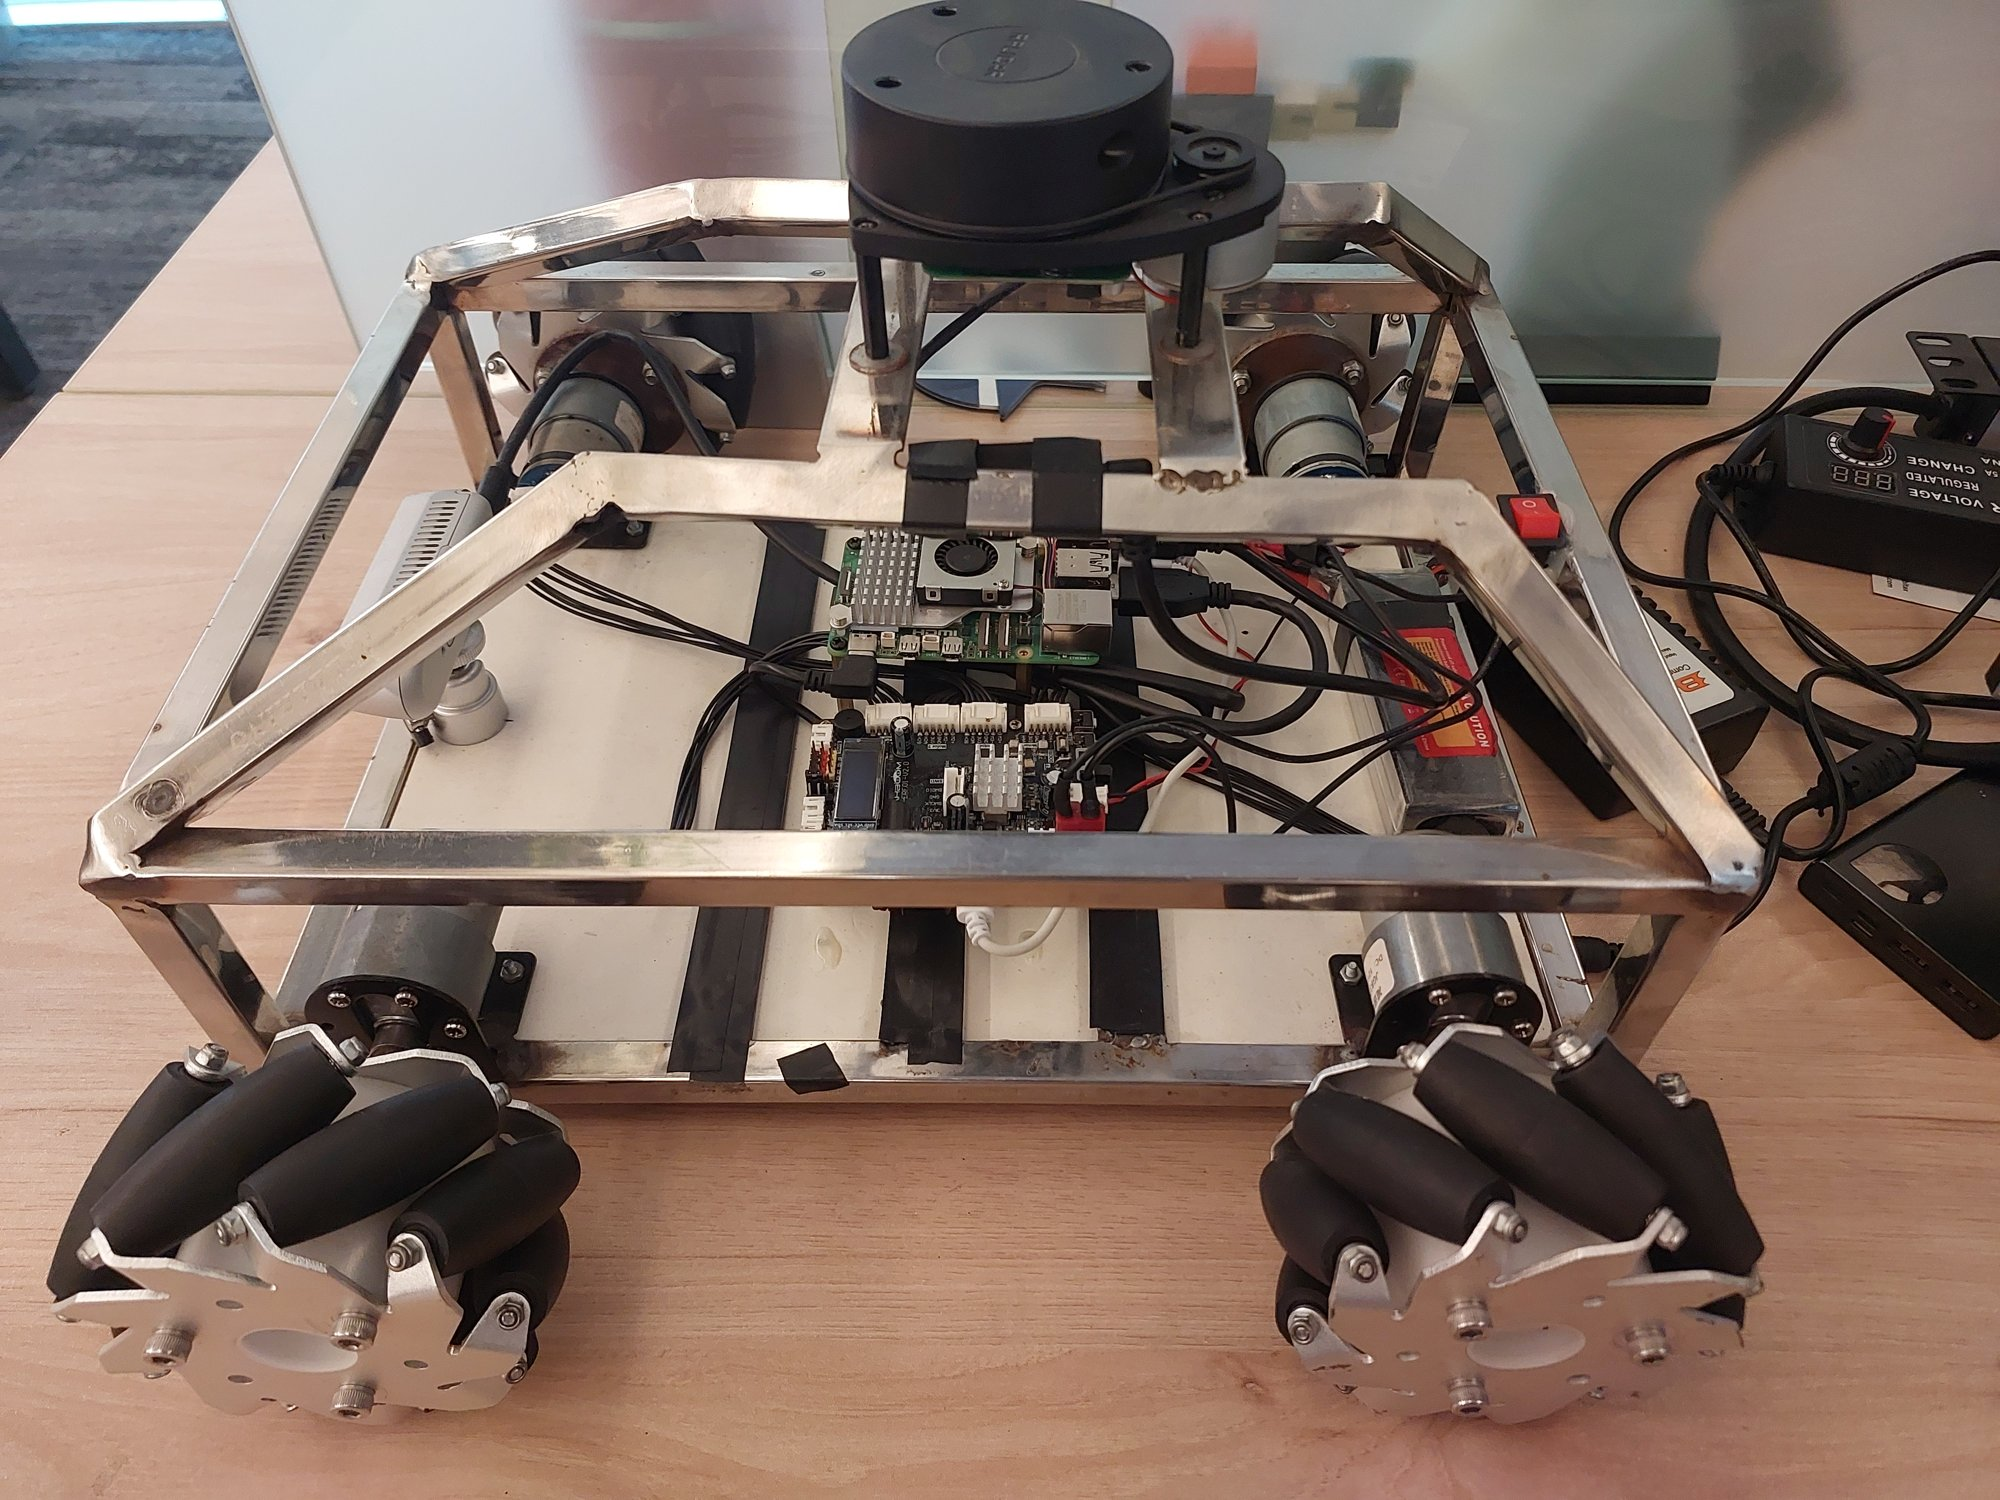
\includegraphics[height=38.5mm]{orbibot-v1-2025-09-24-pi5-build-front.jpg}\hfill
  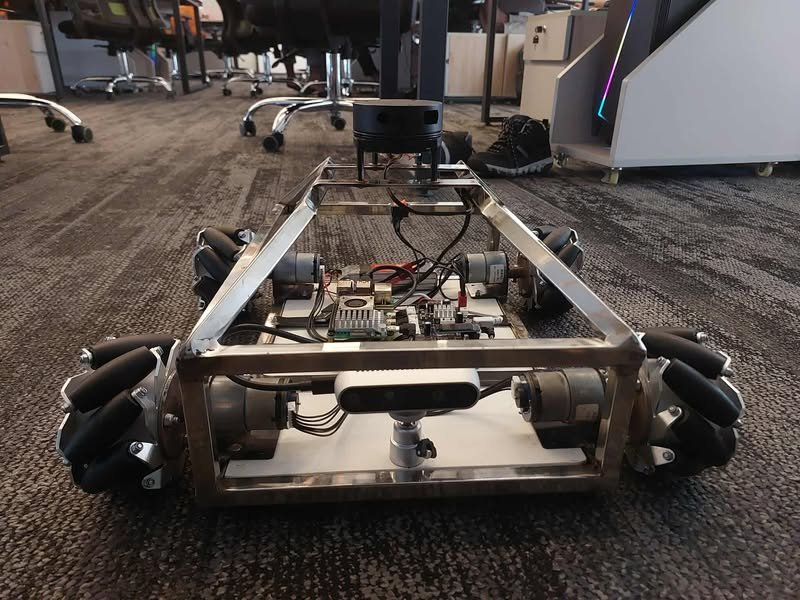
\includegraphics[height=38.5mm]{orbibot-v1-2025-11-25-realsense-front.jpg}\hfill
  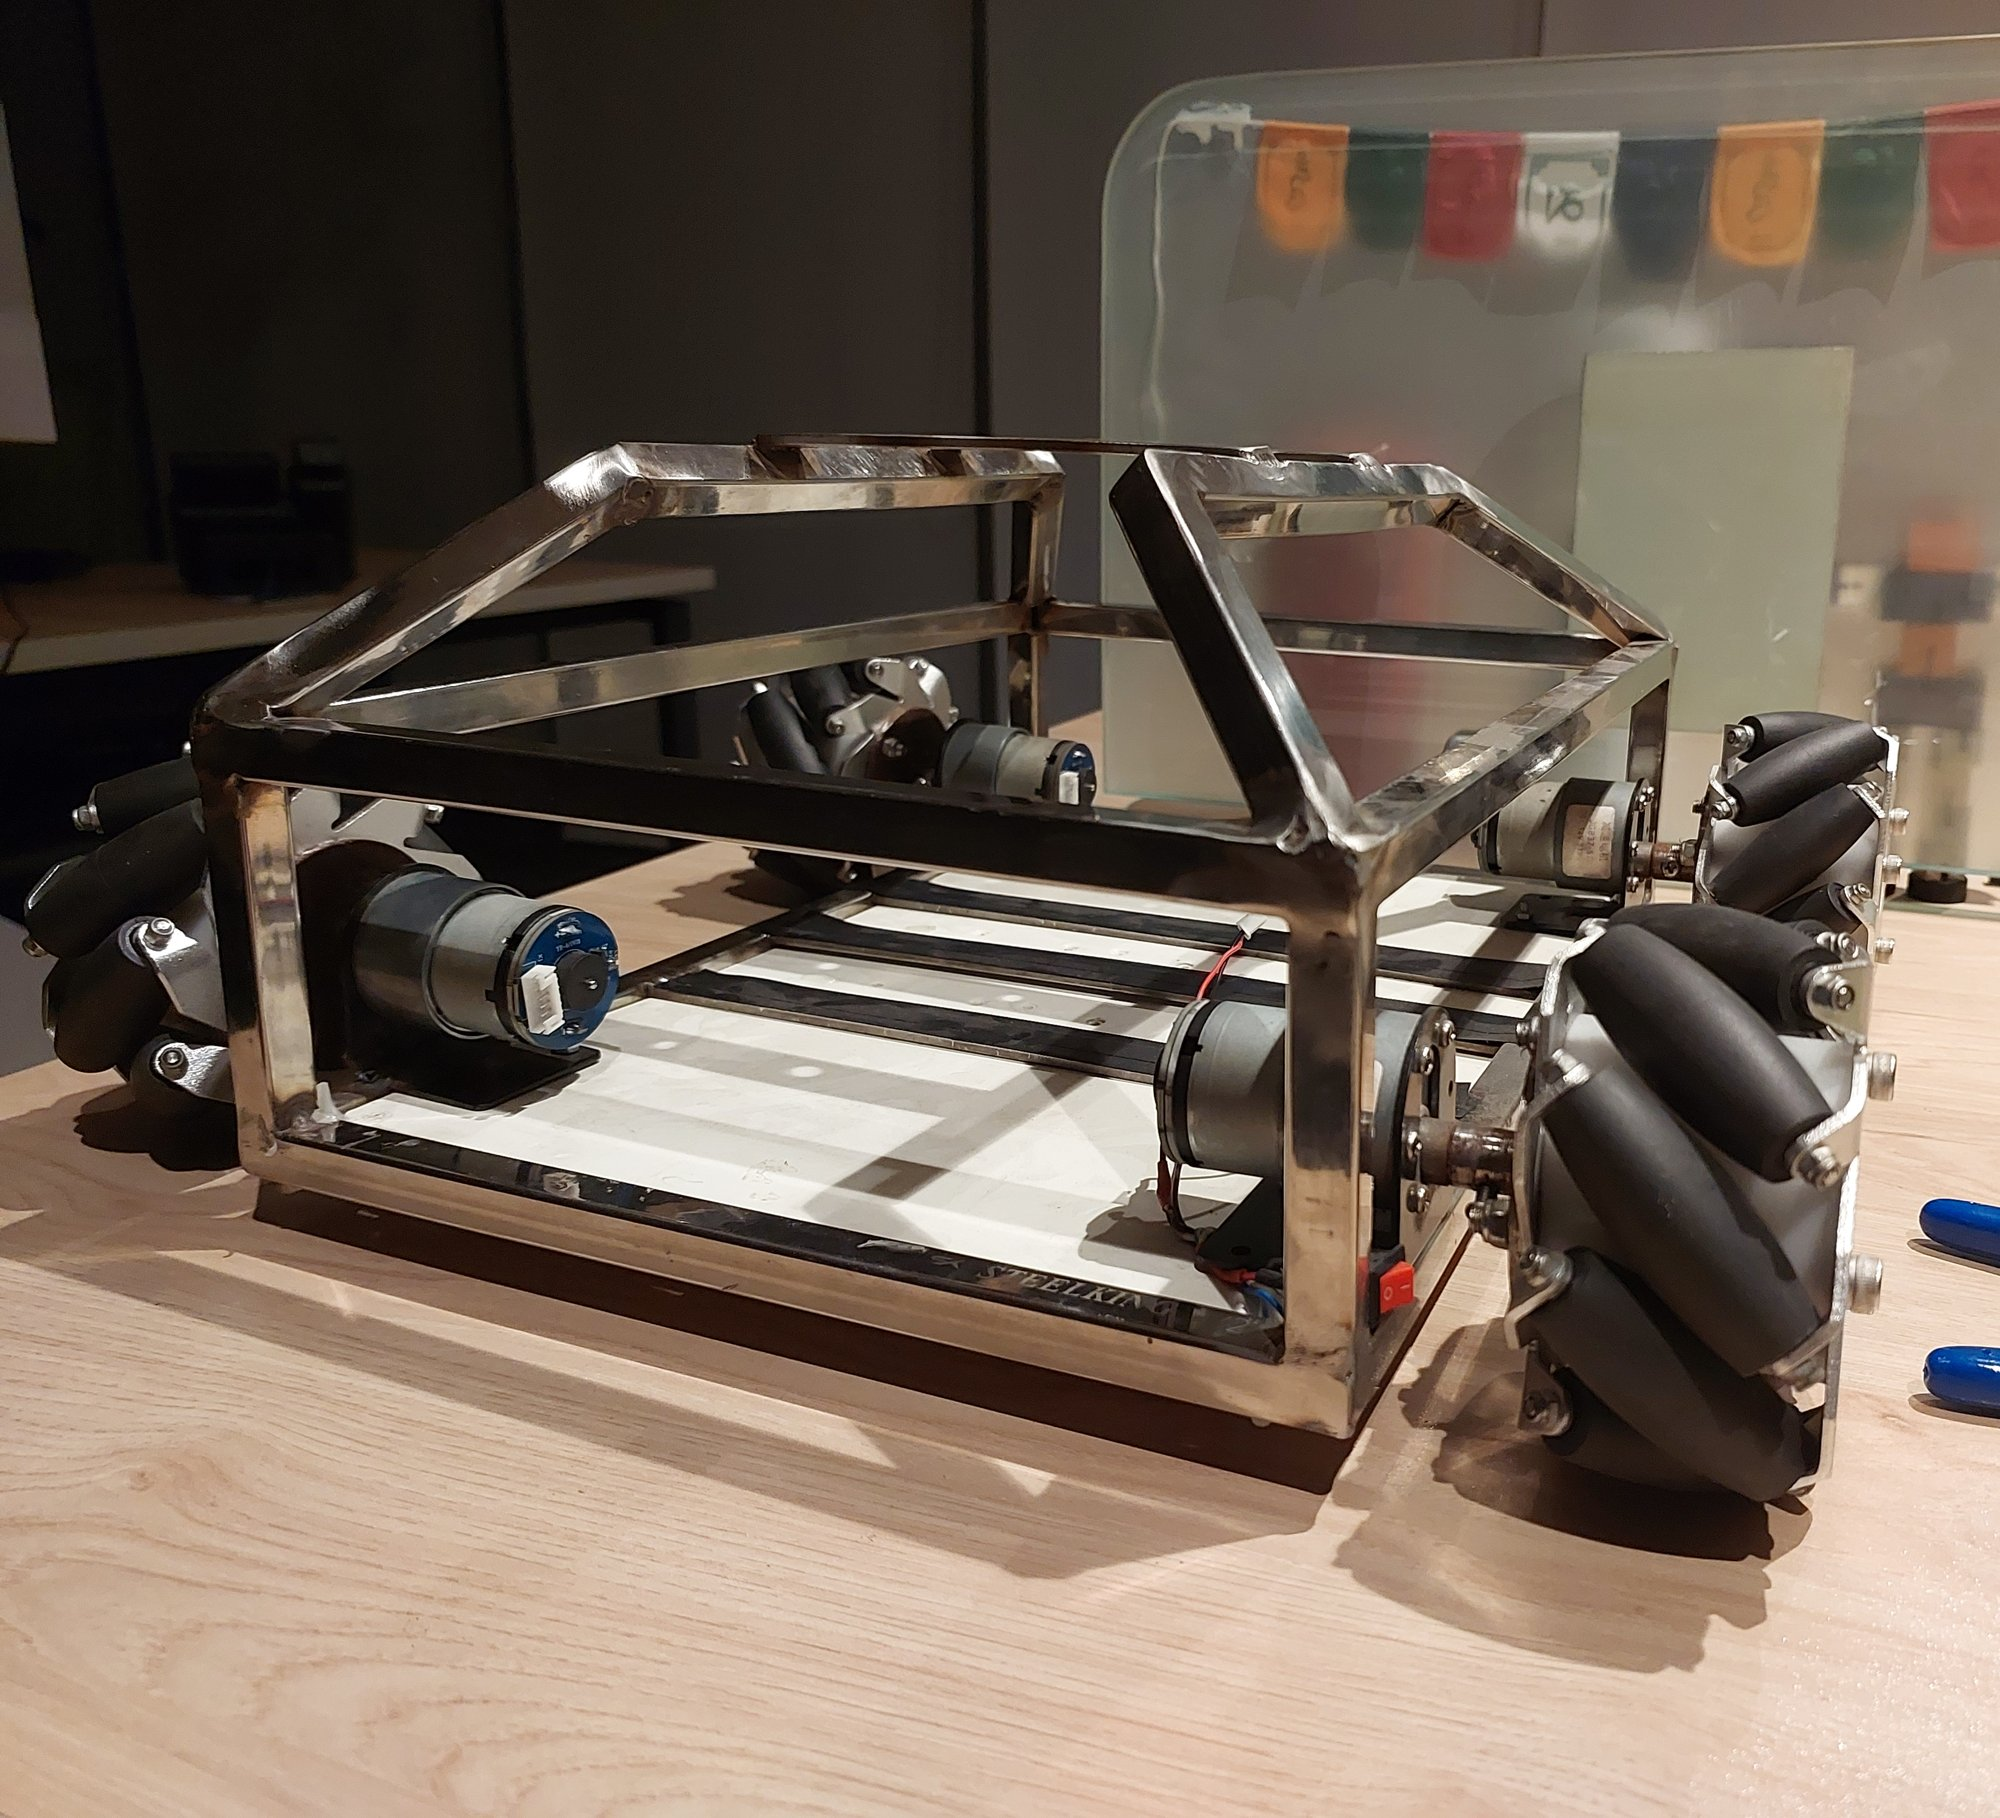
\includegraphics[height=38.5mm]{orbibot-v1-2025-11-06-stripped-frame.jpg}
  \caption{OrbiBot V1. Left: the Raspberry Pi~5 build, with the RPLIDAR A1 on top and the Pi above the motor board (September 2025). Middle: after the rebuild, with the RealSense D435 at the front (November 2025). Right: the welded stainless-steel frame, stripped for the rebuild, with its four JGB37-520 motors and encoders (November 2025).}
  \label{fig:photos}
\end{figure}

The frame is welded stainless steel, 350\,$\times$\,250\,mm in the robot model, on four 100\,mm steel mecanum wheels in an ABBA layout (Fig.~\ref{fig:photos}). Each wheel is driven by a JGB37-520 geared DC motor (30:1, 333\,rpm at 12\,V with no load) with a Hall-effect quadrature encoder giving 1320 counts per wheel turn. The robot model totals about 8\,kg, 6\,kg of it the frame link; the robot was not weighed.

Table~\ref{tab:hw} lists the parts and Fig.~\ref{fig:power} the power and data paths.

\begin{table}[htbp]
  \centering
  \caption{Main parts: datasheet values, with firmware settings marked (f) and measurements marked (m).}
  \label{tab:hw}
  \renewcommand{\arraystretch}{1.25}
  \small
  \begin{tabularx}{0.92\textwidth}{@{}>{\sffamily\bfseries}p{0.2\textwidth}X@{}}
    \toprule
    \thead{Part} & \thead{Key figures} \\
    \midrule
    Host & Raspberry Pi 5, 8\,GB; 4\,$\times$\,Cortex-A76 at 2.4\,GHz; 49.4\,$^\circ$C at idle (m) \\
    Motor board & Yahboom ROSMaster V3.0, STM32F103RCT6, 256\,KB flash, 48\,KB RAM; 4 AM2857 H-bridges, PWM at 20\,kHz (f) \\
    Motors & 4\,$\times$\,JGB37-520, 12\,V, 30:1, 333\,rpm, 3.3\,kg$\cdot$cm rated \\
    Wheels & 4\,$\times$\,100\,mm steel mecanum, 45$^\circ$ rollers \\
    IMU & ICM-20948 on SPI; gyro $\pm$500\,$^\circ$/s and accelerometer $\pm$2\,g ranges (f); magnetometer unused \\
    LiDAR & RPLIDAR A1, 360$^\circ$, 0.15--12\,m, 5.5\,Hz nominal \\
    Depth camera & Intel RealSense D435 (on a USB~2 link on V1) \\
    Battery & 4S LiFePO4, 12.8\,V nominal, 15.5\,Ah, about 198\,Wh; 100\,A BMS \\
    \bottomrule
  \end{tabularx}
\end{table}

\begin{figure}[htbp]
  \centering
  \diagramw{0.88}{figures/fig02-hardware-power}
  \caption{Power (solid lines) and data (dashed). The motor board takes the pack voltage and supplies the Pi over USB-C; the LiDAR and the camera hang off the Pi's USB ports.}
  \label{fig:power}
\end{figure}

Two hardware facts shaped the software.

\begin{itemize}
  \item \textbf{The depth camera ran on a USB~2 link}, at which the D435 cannot deliver depth and colour together at a useful resolution. On V1 the camera launch is off by default, and the dashboard uses only its colour stream.
  \item \textbf{The IMU's magnetometer was removed from use} on 2026-04-28, because indoors the steel frame, motors and battery currents distorted the field enough to make heading worse, not better. The robot therefore has no absolute heading of its own (Section~\ref{sec:ros}).
\end{itemize}

% ---------------------------------------------------------------------------
\section{Firmware}
\label{sec:firmware}

The board ships with closed-source firmware. OrbiBot replaces it with new firmware written in C with PlatformIO, on FreeRTOS~\cite{freertos}. It uses 28.4\,KB of flash (10.9\,\%) and 19.9\,KB of RAM (40.4\,\%), measured with GCC~12.3, so memory is not the limit; CPU time on a Cortex-M3 without a floating-point unit is.

\subsection{Tasks}

Four tasks share the processor (Fig.~\ref{fig:tasks}):

\begin{itemize}
  \item the \textbf{control task}, at 100\,Hz with the highest priority, reads the four encoders, runs one PID loop per wheel, writes the PWM and integrates odometry;
  \item the \textbf{IMU task} reads the gyro and accelerometer at 50\,Hz;
  \item the \textbf{communication task} ticks every millisecond, parses incoming commands and sends five report types, each at 50\,Hz;
  \item the \textbf{monitoring task}, at 1\,Hz, reads the battery, drives the buzzer and feeds a 5\,s independent watchdog only when every other task has shown it is alive.
\end{itemize}

\begin{figure}[htbp]
  \centering
  \diagramw{0.82}{figures/fig03-firmware-tasks}
  \caption{Firmware tasks and the path of a motion command. If no command arrives for 2\,s, the control task stops the motors.}
  \label{fig:tasks}
\end{figure}

\subsection{Speed control}

Each wheel has an incremental PID controller:
\begin{equation}
\Delta u_k = K_p (e_k - e_{k-1}) + \tfrac{K_i}{2}(e_k + e_{k-1}) + K_d (e_k - 2e_{k-1} + e_{k-2}), \qquad u_k = u_{k-1} + \Delta u_k ,
\end{equation}
with default gains $K_p = 0.8$, $K_i = 0.06$, $K_d = 0.5$, which can be changed over the serial link and stored in flash. A conditional clamp at $\pm 4000$ stops the integral term from winding up when the output is saturated in the direction of the error.

The H-bridges have a dead band, which the firmware crosses by adding a fixed offset of 1600 (of 3600) to any non-zero PWM. Section~\ref{sec:limits} shows what this costs at very low speed.

\subsection{Protocol}

The host and the board exchange binary frames compatible with the vendor's protocol, so that existing tools still work (frame format in Appendix, Fig.~\ref{fig:packet}). The host sends motion commands $(v_x, v_y, \omega)$ as 16-bit integers, PID gains, resets, buzzer commands and version requests. The firmware reports speed and battery voltage, raw IMU data, attitude, the four encoder counts and odometry. At 115200\,baud the five report streams use about a third of the link.

\subsection{Safety in the firmware}

The firmware enforces its own limits whatever the host sends:

\begin{itemize}
  \item it clamps commands to 1.0\,m/s and 2.0\,rad/s;
  \item it stops the motors 2\,s after the last command, so a crashed host or a closed browser tab cannot leave the robot driving;
  \item a reset-state command stops the motors at once;
  \item it warns at 11.0\,V and locks the motors out at 10.5\,V;
  \item the watchdog resets the processor if a task hangs.
\end{itemize}

These limits apply to every source of commands, including those that bypass the agent's safety manager (Section~\ref{sec:agent}). Fig.~\ref{fig:safety} places them among the other safety layers.

% ---------------------------------------------------------------------------
\section{Kinematics and Odometry}
\label{sec:kinematics}

With $x$ forward, $y$ to the left, wheel radius $r = 50$\,mm, half-wheelbase $l_x = 130$\,mm and half-track $l_y = 180$\,mm (Fig.~\ref{fig:mecanum}), the firmware converts a body velocity into wheel speeds with the standard inverse kinematics of a mecanum base~\cite{muir1987kinematic}:
\begin{equation}
\begin{bmatrix} \omega_{FL} \\ \omega_{FR} \\ \omega_{BL} \\ \omega_{BR} \end{bmatrix}
= \frac{1}{r}
\begin{bmatrix} 1 & -1 & -(l_x + l_y) \\ 1 & 1 & l_x + l_y \\ 1 & 1 & -(l_x + l_y) \\ 1 & -1 & l_x + l_y \end{bmatrix}
\begin{bmatrix} v_x \\ v_y \\ \omega \end{bmatrix}.
\end{equation}
Odometry uses the matching forward kinematics, integrated at 100\,Hz:
\begin{equation}
v_x = \tfrac{r}{4}\textstyle\sum_i \omega_i, \qquad
v_y = \tfrac{r}{4}(-\omega_{FL} + \omega_{FR} + \omega_{BL} - \omega_{BR}), \qquad
\omega = \tfrac{r}{4(l_x+l_y)}(-\omega_{FL} + \omega_{FR} - \omega_{BL} + \omega_{BR}).
\end{equation}

\begin{figure}[htbp]
  \centering
  \diagramw{0.55}{figures/fig05-mecanum}
  \caption{Top view of the base, to scale. The wheels stand outside the frame (350\,$\times$\,250\,mm in the robot model); roller directions are drawn schematically, as seen from above.}
  \label{fig:mecanum}
\end{figure}

% ---------------------------------------------------------------------------
\section{ROS 2 Software}
\label{sec:ros}

Twelve ROS~2 packages run on the host: the serial bridge, custom messages, the robot model, sensors, localisation, SLAM, navigation, exploration, launch files, the web dashboard, the agent, and a gamepad driver now switched off. Fig.~\ref{fig:rosgraph} shows how the main ones connect.

\begin{figure}[htbp]
  \centering
  \diagramw{1.0}{figures/fig06-ros-graph}
  \caption{Main ROS~2 packages and topics. The dashboard, the agent and Nav2 write \topic{/cmd_vel} (red), and the switched-off gamepad driver is still wired to it; nothing arbitrates between the four (Section~\ref{sec:limits}).}
  \label{fig:rosgraph}
\end{figure}

\paragraph{The bridge} The serial bridge, \topic{orbibot_hardware}, turns the firmware's reports into the topics \topic{/odom}, \topic{/imu/data_raw} and \topic{/joint_states} and into status topics, and turns \topic{/cmd_vel} into motion frames. Its driver started from the vendor's Python library.

\paragraph{Estimation} A Madgwick filter~\cite{madgwick2010} runs in six-axis mode, without the magnetometer, and an EKF~\cite{moore2014ekf} fuses its output with wheel odometry to publish \topic{odom -> base_footprint} (Fig.~\ref{fig:estimation}). Because there is no absolute heading, the EKF takes the IMU's yaw in relative mode, and yaw drift is corrected higher up, by slam\_toolbox or AMCL through \topic{map -> odom}. Exactly one of the two publishes that transform at any time (transform tree in Appendix, Fig.~\ref{fig:tf}).

\begin{figure}[htbp]
  \centering
  \diagramw{0.95}{figures/fig08-estimation}
  \caption{State estimation. With no magnetometer, the map corrects heading.}
  \label{fig:estimation}
\end{figure}

\paragraph{Mapping and navigation} slam\_toolbox~\cite{macenski2021slam} builds maps from the RPLIDAR A1, used to 8\,m. Nav2~\cite{macenski2020nav2} runs with AMCL on saved maps and the MPPI controller~\cite{williams2017mppi} in its omnidirectional (\topic{Omni}) motion model, which lets the planner use the base's sideways motion. A velocity smoother and a collision monitor sit between the controller and the wheels (Appendix, Fig.~\ref{fig:nav}). Nav2 is limited to 0.5\,m/s on each of $x$ and $y$ and to 1.5\,rad/s in rotation.

\paragraph{Exploration} A frontier explorer, a Python re-implementation of the breadth-first frontier search of m-explore-ros2~\cite{mexplore,yamauchi1997frontier}, is written to send goals to Nav2, but has not been tested against a tuned Nav2.

% ---------------------------------------------------------------------------
\section{Web Dashboard}
\label{sec:dashboard}

A React and TypeScript dashboard (Fig.~\ref{fig:dash}) shows the battery, the four motors, odometry, the IMU, the LiDAR, the live map and the camera. It drives the base with on-screen controls or the keyboard, sets Nav2 goals and tunes the PID gains.

\begin{figure}[htbp]
  \centering
  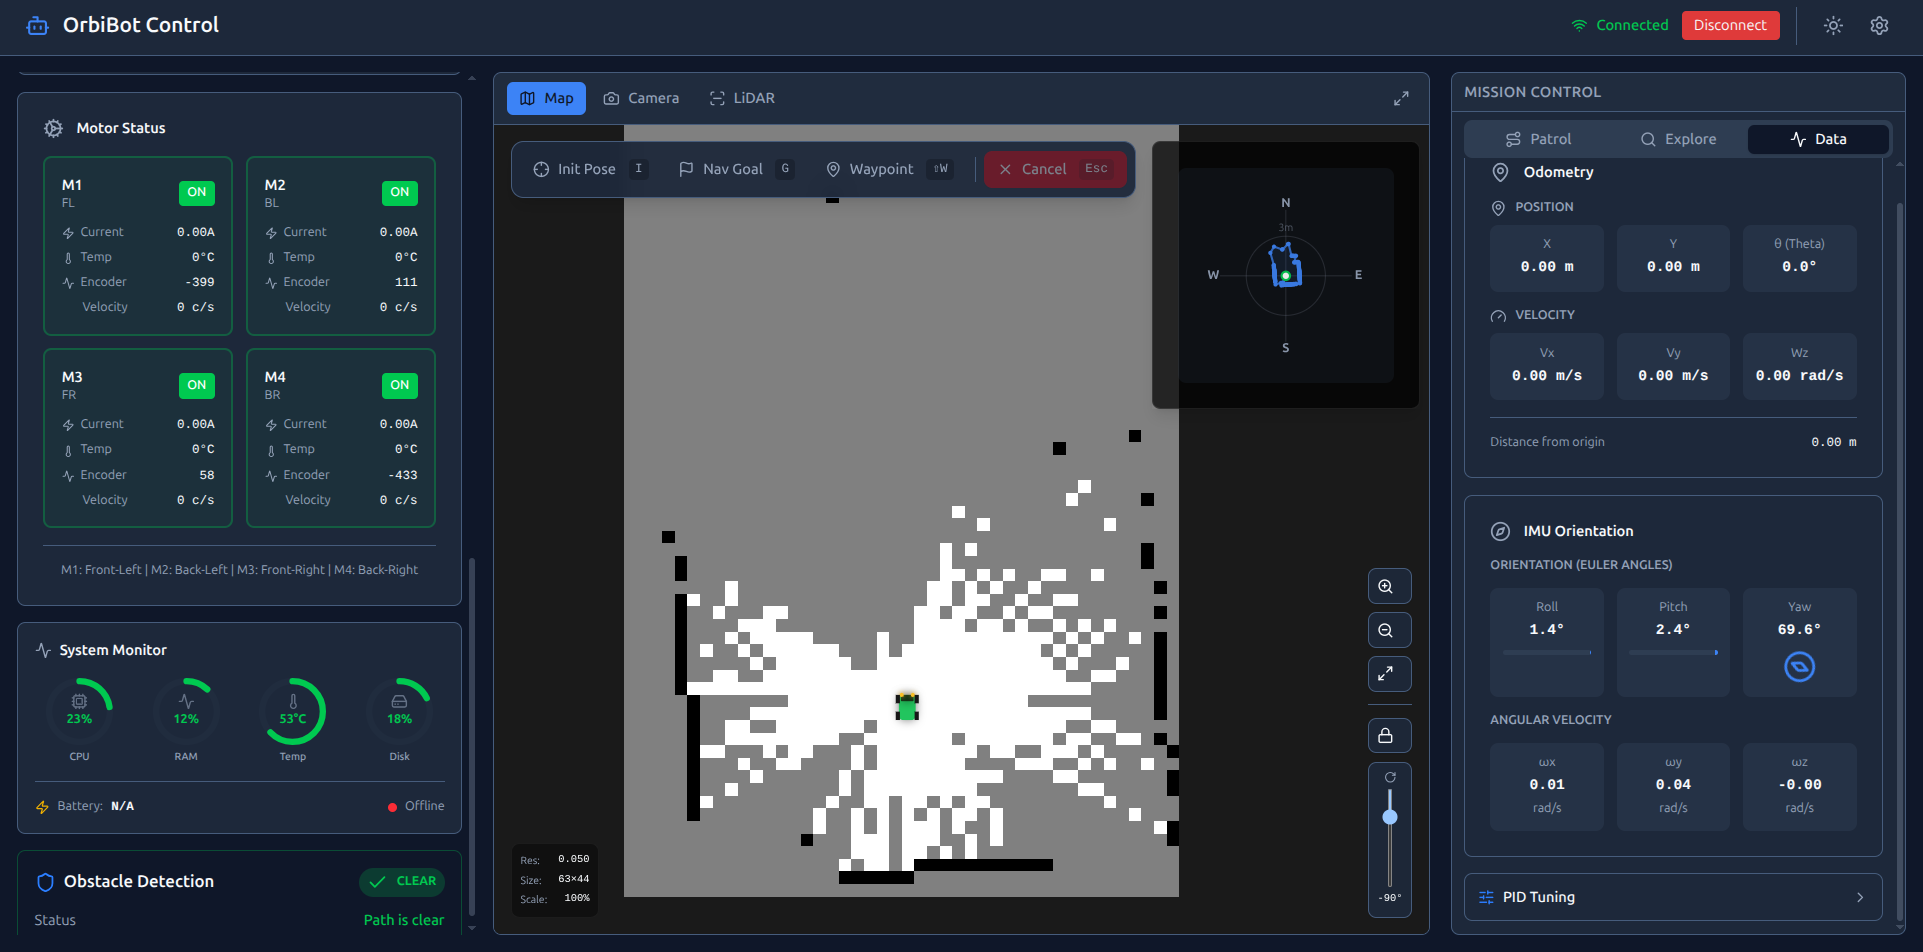
\includegraphics[width=0.9\textwidth]{orbibot-v1-web-dashboard.png}
  \caption{The dashboard: motor status, system monitor, the SLAM map, odometry and IMU orientation.}
  \label{fig:dash}
\end{figure}

It reaches ROS~2 through rosbridge~\cite{crick2017rosbridge} as JSON over a WebSocket. The camera takes a separate path: a WebRTC server, itself a ROS~2 node, subscribes to the colour image topic and streams it to the browser as video, so camera frames never pass through rosbridge (Appendix, Fig.~\ref{fig:dashpath}). The dashboard never drives hardware directly: its commands use the same topics as every other client.

Building it showed that the cost of a robot dashboard is not drawing, which happens in the operator's browser, but what the robot must serialise and send: each of about fifteen subscriptions is turned into JSON separately on the Pi. A cheaper design, with one packed telemetry message, a decimated scan, a map sent on request and a camera path that skips ROS~2 entirely, is drawn up but not built.

% ---------------------------------------------------------------------------
\section{LLM Agent}
\label{sec:agent}

\topic{orbibot_agent} lets a language model operate the robot through tools (Fig.~\ref{fig:agent}). It works with Google Gemini, Anthropic Claude, Moonshot Kimi, or a local model served by Ollama, behind one provider interface with streaming. An orchestrator sends the user's message and the tool schemas to the model, executes the tool calls it returns, and feeds the results back, for up to ten rounds (sequence in Appendix, Fig.~\ref{fig:seq}).

\begin{figure}[htbp]
  \centering
  \diagramw{0.95}{figures/fig12-agent}
  \caption{The agent. The HTTP and terminal interfaces share one orchestrator; the MCP server hands the tools straight to the client's own model. The 58 tools in seven groups reach ROS~2 directly through \topic{rclpy}; the two direct motion tools pass the safety manager first.}
  \label{fig:agent}
\end{figure}

\paragraph{Tools} The 58 tools fall into seven groups: motion (4), sensors (13), firmware (7), generic ROS~2 access (10), navigation and SLAM (19), diagnostics (3) and analysis (2). Each is a typed function with a JSON schema. The agent talks to ROS~2 directly through \topic{rclpy}, not through rosbridge.

\paragraph{Interfaces} An HTTP server with streamed replies, which the dashboard's chat panel uses, and a terminal client both run through the orchestrator. An MCP server over standard input and output exposes the tools directly, so that a general-purpose AI client, whose own model then runs the loop, can work with the robot. On 2026-03-14 the agent itself, driven through this MCP server, ran a baseline check of the robot's health, sensors and firmware, which is kept in the repository; its IMU figures predate the IMU fixes and are not used here.

\paragraph{Safety} The two direct motion tools, \topic{move_robot} and \topic{stop_robot}, pass a safety manager that clamps each linear axis to 0.5\,m/s and rotation to 2.0\,rad/s and caps any single motion at 10\,s. It also checks an emergency-stop flag, but nothing in the code sets that flag yet.

Other tools can move the robot without the safety manager: the Nav2 tools, which fall under Nav2's own limits, and the generic topic-publishing tool, which can write any velocity to \topic{/cmd_vel}. For all of them, the firmware's limits and timeout still apply (Fig.~\ref{fig:safety}). Routing every motion through the safety manager is an open fix.

\begin{figure}[htbp]
  \centering
  \diagramw{0.85}{figures/fig14-safety-layers}
  \caption{Safety layers, and how far each has been checked.}
  \label{fig:safety}
\end{figure}

% ---------------------------------------------------------------------------
\section{Bench Evaluation}
\label{sec:eval}

All motion tests were run with the robot raised and the wheels free to spin, on 2026-04-19 and 2026-04-28. Test scripts on the host sent commands straight over the serial link and logged the firmware's reports; static sensor checks followed on 2026-08-03.

These tests check directions, signs, tracking and safety behaviour. They cannot check distance, drift or traction, which need the robot on the floor. The full procedures and logs are in the firmware test report~\cite{orbibotrepo}.

\subsection{Kinematics and velocity tracking}

Each of four motions was commanded for 2\,s, re-sent every 100\,ms. All four wheel-direction patterns matched the inverse kinematics, so no motor or encoder was wired backwards.

Table~\ref{tab:kin} and Fig.~\ref{fig:vel} give the measured chassis velocity. Forward, backward and turning were within 4.1\,\% of the command; sideways motion reached 90.7\,\%, and the off-axis components stayed below 20\,mm/s or mrad/s.

\begin{table}[htbp]
  \centering
  \caption{Commanded and measured chassis velocity, 2\,s runs, wheels off the ground (2026-04-19). Units: mm/s and mrad/s.}
  \label{tab:kin}
  \renewcommand{\arraystretch}{1.25}
  \begin{tabular}{@{}lrrrr@{}}
    \toprule
    \thead{Motion} & \thead{Command} & \thead{$v_x$} & \thead{$v_y$} & \thead{$\omega$} \\
    \midrule
    Forward  & $v_x = 150$   & 148  & 17  & $-19$ \\
    Backward & $v_x = -150$  & $-154$ & 0 & 0 \\
    Sideways & $v_y = 150$   & $-5$ & 136 & 19 \\
    Turning  & $\omega = 700$ & 0   & $-11$ & 729 \\
    \bottomrule
  \end{tabular}
\end{table}

\begin{figure}[htbp]
  \centering
  % Measured chassis velocity as a share of the command, wheels off the ground,
% 2 s runs, 2026-04-19 (firmware test report, section 6). 100 % = the command.
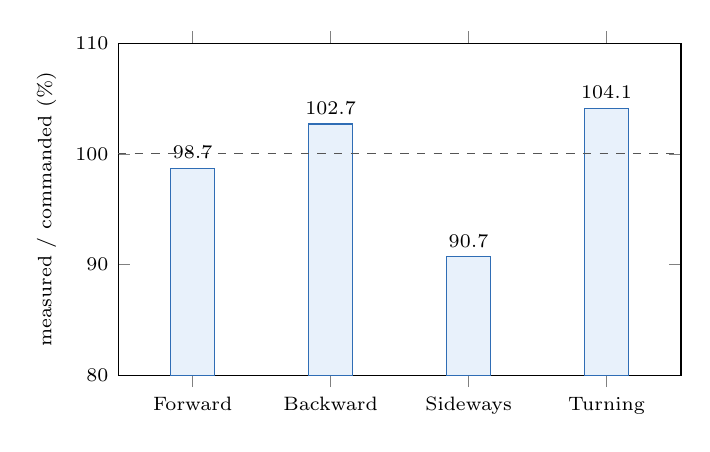
\begin{tikzpicture}
  \begin{axis}[
      ybar, bar width=16pt, width=0.72\textwidth, height=58mm,
      ymin=80, ymax=110, ylabel={measured / commanded (\%)},
      symbolic x coords={Forward, Backward, Sideways, Turning},
      xtick=data, tick label style={font=\scriptsize}, label style={font=\scriptsize},
      nodes near coords, nodes near coords style={font=\scriptsize},
      enlarge x limits=0.18]
    \addplot[fill=mcu, draw=mcuedge] coordinates {(Forward,98.7) (Backward,102.7) (Sideways,90.7) (Turning,104.1)};
    \draw[dashed, hwedge] (rel axis cs:0,0.6667) -- (rel axis cs:1,0.6667);
  \end{axis}
\end{tikzpicture}

  \caption{Measured chassis velocity as a share of the command (dashed line: 100\,\%).}
  \label{fig:vel}
\end{figure}

In the same runs the back-right encoder counted about 9--16\,\% fewer ticks than the others. A later run at the 1.0\,m/s limit, 5\,s long with about 250 samples per motor, showed no weak motor at steady state: once the loops converged, the four wheels averaged 1001.7 to 1002.5\,mm/s, 0.1\,\% apart (Fig.~\ref{fig:motors}). The test report attributes the earlier gap to start-up stiction in that drivetrain.

\begin{figure}[htbp]
  \centering
  % Mean wheel speed per motor at the 1.0 m/s firmware limit, with one standard
% deviation, about 250 samples each, wheels off the ground, 2026-04-28 (section 9.2).
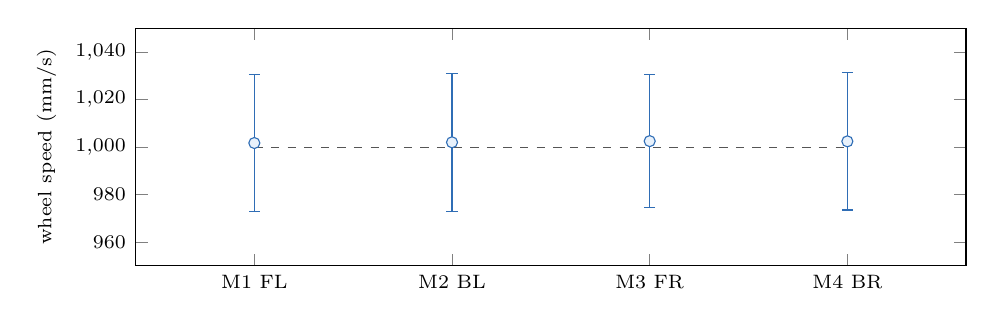
\begin{tikzpicture}
  \begin{axis}[
      width=\columnwidth, height=46mm,
      ymin=950, ymax=1050, ylabel={wheel speed (mm/s)},
      symbolic x coords={M1 FL, M2 BL, M3 FR, M4 BR},
      xtick=data, tick label style={font=\scriptsize}, label style={font=\scriptsize},
      enlarge x limits=0.2]
    \addplot[only marks, mark=*, mark options={fill=mcu, draw=mcuedge}, color=mcuedge,
             error bars/.cd, y dir=both, y explicit]
      coordinates {(M1 FL,1001.7) +- (0,28.7) (M2 BL,1002.0) +- (0,29.1)
                   (M3 FR,1002.5) +- (0,28.0) (M4 BR,1002.4) +- (0,28.9)};
    \addplot[dashed, hwedge] coordinates {(M1 FL,1000) (M4 BR,1000)};
  \end{axis}
\end{tikzpicture}

  \caption{Mean wheel speed at the 1.0\,m/s limit, with one standard deviation (2026-04-28).}
  \label{fig:motors}
\end{figure}

\subsection{Safety behaviour}

A single command of 0.1\,m/s was sent and nothing after it. The firmware reported motion until 1.82\,s and zero from 2.12\,s on (Fig.~\ref{fig:timeout}). With reports every 0.3\,s in this log, the stop falls between those two samples, on the 2\,s setting.

\begin{figure}[htbp]
  \centering
  % One MOTION command of 0.1 m/s at t = 0 and nothing after it. The firmware
% reports zero from t = 2.12 s on. Wheels off the ground, 2026-04-19 (section 7.1).
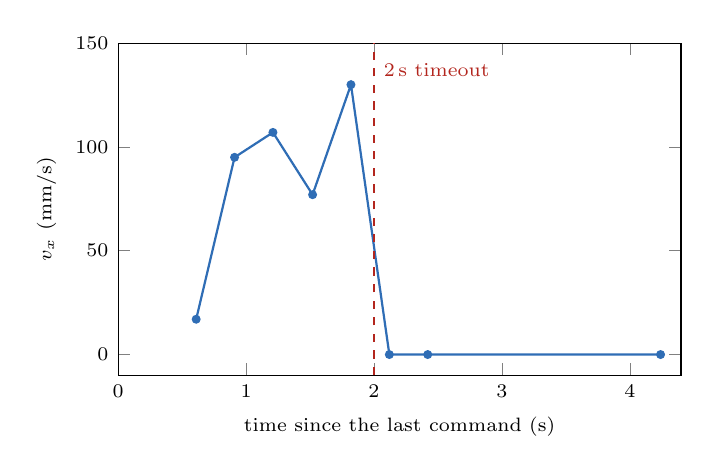
\begin{tikzpicture}
  \begin{axis}[
      width=0.72\textwidth, height=58mm,
      xmin=0, xmax=4.4, ymin=-10, ymax=150,
      xlabel={time since the last command (s)}, ylabel={$v_x$ (mm/s)},
      tick label style={font=\scriptsize}, label style={font=\scriptsize}]
    \addplot[thick, mcuedge, mark=*, mark size=1.2pt] coordinates {
      (0.61,17) (0.91,95) (1.21,107) (1.52,77) (1.82,130) (2.12,0) (2.42,0) (4.24,0)};
    \draw[dashed, warnedge] (axis cs:2.0,-10) -- (axis cs:2.0,150)
      node[pos=0.92, right, font=\scriptsize, text=warnedge] {2\,s timeout};
  \end{axis}
\end{tikzpicture}

  \caption{Command timeout: one 0.1\,m/s command at $t = 0$, then silence (2026-04-19).}
  \label{fig:timeout}
\end{figure}

A command of 3\,m/s, three times the limit, produced a peak of 1023\,mm/s; the 2.0\,rad/s rotation clamp was not exercised. A reset-state command during motion stopped the motors at once. The watchdog fired once, by accident, during the malformed-input test described below, and reset the board as designed. The battery lockout was reviewed in the code but not triggered, since that would mean draining the battery.

\subsection{Serial link and robustness}

With all five reports enabled the firmware sent 270 frames per second, 54\,Hz per type against a 50\,Hz target; the difference comes from the scheduler's tick granularity and is the same for all five streams. Commands were then sent at a target of 500\,Hz, of which the host achieved about 328\,Hz (1083 in 3.30\,s), while 825 reports were parsed, with no checksum error, overflow or torn frame. An unknown function code was dropped without interrupting the stream.

\begin{summarybox}{A critical fault, found and fixed}
A frame with a valid checksum but no payload made the firmware act on stale data in memory:
\begin{itemize}
  \item a truncated motion command drove the wheels at 1029\,mm/s;
  \item a truncated PID command caused a 993\,mm/s spike;
  \item a truncated calibration command froze the reports until the watchdog reset the board.
\end{itemize}
A per-function minimum length check, added before any handler runs, fixed all three. After it, twenty truncated frames of each of five kinds caused no motion and no gap in the reports.
\end{summarybox}

\subsection{Sensors, rates and resources}

With the robot level and still, the accelerometer read $|a| = 9.802$\,m/s$^2$, 0.9995 of standard gravity, after a fix to its Z axis on 2026-08-03; X and Y read 14 and 16\,mm/s$^2$. The gyro's Z axis showed a bias of $-15$\,mrad/s (0.86\,$^\circ$/s) in April. On the same day as the accelerometer fix, the full chain from firmware to ROS~2 delivered \topic{/imu/data_raw}, \topic{/joint_states} and \topic{/orbibot/encoders} at about 50\,Hz.

\subsection{What was run but not measured}

Several parts of the system were used on the robot but produced no numbers:

\begin{itemize}
  \item \textbf{on video:} maps built with slam\_toolbox while driving (from July 2025), localising and driving on a saved map of a home (January 2026), and driving from the dashboard with the live camera and map (February 2026);
  \item \textbf{in the project's status notes only:} Nav2 set up and run in a small room (March 2026), and the agent running on the robot behind the dashboard.
\end{itemize}

They show that the pieces work together; they do not show how well.

% ---------------------------------------------------------------------------
\section{Limitations}
\label{sec:limits}

\paragraph{Nothing measured on the floor} Distance, drift, traction, PID under load, Nav2's success rate and path quality, and the agent's task success are all unmeasured. The 1.74\,m/s top speed is worked out from the motor datasheet; the firmware caps the robot at 1.0\,m/s.

\paragraph{No command arbitration} The dashboard, the agent and Nav2's collision monitor all publish \topic{/cmd_vel} (the switched-off gamepad driver is still wired to it), and the last writer wins. A Nav2 goal and the dashboard's joystick can fight mid-drive, and closing the dashboard mid-command leaves the last velocity in force until the firmware's 2\,s timeout. A fix with \topic{twist_mux}, priorities and per-source timeouts is designed but not built (Appendix, Fig.~\ref{fig:mux}).

\paragraph{Agent safety has gaps} Only the agent's two direct motion tools pass its safety manager; its Nav2 tools and its generic topic-publishing tool do not, and its emergency-stop flag is never set. The firmware's clamp and timeout are the only limits common to every path.

\paragraph{Estimation data before August 2026 is suspect} Two faults fed the estimator bad data for months: the accelerometer read too high on Z, and raw IMU packets were silently dropped by a length check whenever the firmware and driver were out of step. Any tuning or drift figure recorded before 2026-08-03 should be measured again; the EKF must be re-tuned.

\paragraph{No absolute heading} Without the magnetometer, yaw comes from the gyro alone between map corrections; its drift rate has not been measured.

\paragraph{Very low speeds} Below about 50\,mm/s per wheel the fixed dead-band offset makes the wheels uneven: at 30\,mm/s for 2.5\,s the encoders counted 54, 351, 407 and 0 ticks against about 315 expected (the firmware test report first gave 158, an arithmetic slip since corrected). Navigation speeds are unaffected, but a planner's slow final approach could be.

\paragraph{Other limits} The accelerometer's X and Y scale has not been checked under a known acceleration; storing PID gains in flash across a reboot was not exercised; the depth camera ran on USB~2; and Nav2's footprint and inflation were never measured.

% ---------------------------------------------------------------------------
\section{Lessons Learned}

\paragraph{Put deadlines on the microcontroller} Keeping every timed loop and every stop condition in the firmware meant each could be tested on its own, from a script, with no ROS~2 stack running; whether the split also holds under heavy host load is still to be measured.

\paragraph{Test what the parser does with bad input} The most dangerous fault found was not in control but in parsing: a well-formed but empty frame made the wheels move.

\paragraph{A 2D LiDAR sees one slice} A table top above the scan plane or a low box below it is invisible to the map, which is why the depth camera was added.

\paragraph{Write down what was measured} Recording each test with its date, conditions and limits is what made it possible to see that months of estimator tuning rested on faulty IMU data, and to say so here.

% ---------------------------------------------------------------------------
\section{Conclusion and Future Work}

OrbiBot V1 shows that a hand-built mecanum robot on a Raspberry Pi~5 and a commercial STM32 board can carry the full ROS~2 navigation stack and an LLM agent, if the microcontroller keeps every deadline and enforces its own safety limits. The bench tests confirm the firmware's kinematics, tracking, linear speed limit and timeout, and found and fixed one critical parsing fault.

The measurements that would close the gaps in Section~\ref{sec:limits} are floor tests: odometry drift on closed square paths, Nav2's success rate and time over a fixed set of goals, the agent's success rate on a fixed set of natural-language tasks across model providers, and wheel behaviour under heavy host load. Command arbitration, and routing all of the agent's motion through its safety manager, would come before any of them.

% ---------------------------------------------------------------------------
\section*{Acknowledgements}

The firmware keeps a protocol compatible with Yahboom's, and the serial driver started from Yahboom's library. The firmware uses FreeRTOS, ST's STM32F10x Standard Peripheral Library, ARM's CMSIS and the font table of stm32-ssd1306 by Aleksander Alekseev, with their notices kept; its SSD1306 display routines follow an existing driver's interface, whose source is still being traced. The dashboard uses shadcn/ui components (MIT). Three wheel and LiDAR meshes in the robot model are third-party CAD whose source was not recorded. Design ideas came from LGDXRobot2 and AuBot.

Parts of the firmware audit, its bench tests and this documentation were carried out with AI coding assistants under the author's direction; every result reported here was checked against the logged data and the code.

{\small
\bibliographystyle{IEEEtran}
\bibliography{references}
}

% ---------------------------------------------------------------------------
\clearpage
\appendix
\section{Additional Diagrams}

\begin{figure}[htbp]
  \centering
  \diagramw{0.9}{figures/fig15-timeline}
  \caption{Build timeline, from the dated photos, videos, test reports and status notes. Green: robot and ROS~2; orange: dashboard; blue: firmware.}
  \label{fig:timeline}
\end{figure}

\begin{figure}[htbp]
  \centering
  \diagramw{0.85}{figures/fig04-packet-format}
  \caption{Serial frame, with a version request and its reply as recorded on the robot.}
  \label{fig:packet}
\end{figure}

\begin{figure}[htbp]
  \centering
  \diagramw{0.6}{figures/fig07-tf-tree}
  \caption{Transform tree; the base frame is \topic{base_footprint}.}
  \label{fig:tf}
\end{figure}

\begin{figure}[htbp]
  \centering
  \diagramw{0.95}{figures/fig09-navigation}
  \caption{Nav2's command chain on V1.}
  \label{fig:nav}
\end{figure}

\begin{figure}[htbp]
  \centering
  \diagramw{0.9}{figures/fig11-dashboard}
  \caption{Dashboard data paths as built.}
  \label{fig:dashpath}
\end{figure}

\begin{figure}[htbp]
  \centering
  \diagramw{0.85}{figures/fig13-tool-call-sequence}
  \caption{One request through the agent.}
  \label{fig:seq}
\end{figure}

\begin{figure}[htbp]
  \centering
  \diagramw{0.7}{figures/fig10-command-arbitration}
  \caption{Velocity commands: (a) as built; (b) the designed fix, with priority and timeout per source.}
  \label{fig:mux}
\end{figure}

\end{document}
